\chapter{Metabolism Is a Network, Not an Assembly Line}

\begin{kaichang}
Dinner is ready: rice, scrambled eggs, some greens, and a piece of braised pork. Before picking up your chopsticks, consider this chapter's question: \textbf{where will this meal be three days from now?}

Write down your guess, preferably with proportions. Perhaps thirty percent becomes muscle, forty percent is burned for energy, twenty percent is stored as fat, and ten percent leaves the body. Which destination takes the largest share? Is braised pork especially likely to become your own flesh?

We will return to your answer at the end. The right answer is almost certainly ``a little of everything,'' and the destinations depend less on what the meal is than on a vast, constantly self-adjusting network inside you. That network is \textbf{metabolism}.
\end{kaichang}

\section{Phenomena: Where Did the Meal Go?}

Leave molecules aside for now and consider observable facts.

Half an hour after eating, hunger fades and you feel slightly warmer: digestion, absorption, and transport themselves cost energy. An hour after the meal, pricking your finger with a glucose meter, which many people with diabetes have at home, would show a rise in blood glucose. Two hours later, it returns to its premeal level. The next morning, your weight is not much different: much of the meal has quietly left in exhaled air, sweat, and urine, while some was never absorbed and simply passed through your gut.

\textbf{Translator safety note:} Do not prick fingers or borrow a family member's glucose-testing equipment for this lesson; use published example readings. Lancets and fingerstick devices must not be shared, even with a new blade, because infections can spread. See \href{https://www.fda.gov/regulatory-information/search-fda-guidance-documents/blood-lancet-labeling-guidance-industry-and-food-and-drug-administration-staff}{FDA blood-lancet guidance}.

Eat more than you expend for several weeks, and weight gradually rises; the reverse makes it fall. Strenuous exercise deepens and accelerates breathing. Going a long time without food causes dizziness, palpitations, and poor concentration. The white cloud you exhale in winter consists of metabolic water vapor condensing into tiny droplets; urine removes urea and excess salts daily. These are all visible, measurable phenomena. Together, they show that \textbf{food neither disappears nor turns into you unchanged: it continually flows, transforms, enters, and leaves}.

Want direct evidence that transformation is happening? You need no reagent, only your breathing.

\begin{shiyan}
\textbf{Count Your Body Factory's Exhaust Rate}

Materials: a watch or phone with a stopwatch.

Procedure: sit quietly for three minutes, then count and record your breaths over one minute. Walk briskly in place or do squats for two minutes, stop, and immediately count another minute of breathing. Rest for five minutes and count a third time.

Observations: how much did breathing increase after exercise? How many minutes did it take to return to rest? Compared with resting breath, what extra substance are you exhaling?

Safety: stay within your abilities; stop and rest immediately if you feel chest tightness or dizziness. Do not do this within an hour after eating.
\end{shiyan}

Exercise makes breathing deeper and faster because muscles burn fuel faster, and the resulting waste gas, carbon dioxide, must travel from blood to lungs and leave more quickly. What you counted was your body factory's exhaust rate. The factory never shuts down; only its speed changes.

\section{Particles: Two Streets in Opposite Directions}

Zoom to the molecular level. The meal's main cargo consists of three large-molecule classes: starch from Chapter 46, fat from Chapter 47, and protein from Chapter 48. Too large to cross the intestinal wall into blood, they must first be cut into small parts by enzymes: starch into glucose, fat into fatty acids and glycerol, and protein into amino acids. The small intestine absorbs these parts into the blood, which delivers them to every cell.

Inside cells, the parts take streets in two directions.

\textbf{Catabolism} breaks molecules into smaller pieces, harvesting energy and electrons along the way. Glucose becomes pyruvic acid through cytoplasmic glycolysis in Chapter 52, then enters mitochondria and is broken down to carbon dioxide through Chapter 53's citric-acid cycle. Extracted high-energy electrons drive ATP synthesis. Fatty acids too are cut apart two carbons at a time. Large becomes small; energy comes in.

Breaking down amino acids leaves another troublesome part: the nitrogen-containing amino group. Ammonia is toxic to cells and cannot simply be dumped into blood. The liver converts it into less toxic, water-soluble urea, which the kidneys excrete in urine. This is why a high-protein feast makes you thirsty and increases urination: your body is working overtime to handle nitrogen. The blood urea nitrogen entry on a medical report measures this waste-disposal pipeline's workload.

\textbf{Anabolism} spends ATP energy to assemble large molecules from small ones. Glucose becomes glycogen stored in liver and muscle; fatty acids become fat stored in adipose tissue; amino acids become your own proteins, including muscle fibers, hair, enzymes, and antibodies. Small becomes large; energy is spent. Every centimeter of growth, patch of new skin over a wound, and biceps built through months of training is an anabolic construction project.

These streets are not isolated one-way routes. They form a city network: some vehicles go east and others west, with intersections connecting the same neighborhoods. The rest of this chapter tours those intersections.

\begin{qiaoliang}
How much traffic does the network carry? Calculate with ATP, introduced in Chapter 50. An adult with normal daily activity uses about 2000 kilocalories. Under actual cellular conditions, hydrolyzing 1 mole of ATP provides about 12 kilocalories of usable energy, so the body spends roughly $2000 \div 12 \approx 170$ moles daily. One mole weighs about 507 grams, giving a daily synthesized and broken-down total of $170 \times 507 \approx 8.6 \times 10^{4}$ grams, \textbf{more than an adult's body weight}. Yet only about 50 grams, or 0.1 moles, are present at any instant. Each ATP molecule must therefore cycle an average of $170 \div 0.1 \approx 1700$ times daily, completing a discharge--recharge cycle in less than a minute. Energy currency matters for circulation, not hoarding. Metabolism is first an unceasing flow and only second an inventory.
\end{qiaoliang}

\section{Rules: Where the Main Roads Meet}

Chapters 52 and 53 followed glycolysis and the citric-acid cycle. Look down from higher up now: the three major roads for carbohydrates, fats, and proteins converge on the same downtown roundabout.

The key junction is a small molecule called \textbf{acetyl coenzyme A}, which you can imagine as a little freight cart carrying two carbons. Glucose becomes pyruvic acid, then acetyl-CoA. Fatty acids are cut into successive acetyl-CoA units. Many amino acids lose their amino groups and leave carbon skeletons that become acetyl-CoA or enter the citric-acid cycle at intermediate stations. Cargo from three different sources mixes here.

The carts then have two main destinations. They can enter the citric-acid cycle, be fully broken down to \chem{CO_2}, and pass electrons to the respiratory chain to make ATP: burning. Or they can supply construction sites: acetyl-CoA starts fatty-acid and cholesterol synthesis, while cycle intermediates provide amino-acid skeletons that are assembled into proteins: building.

The junction works both ways. Sugar can become fat, which is why excess rice and noodles can add body fat. During fasting, amino acids can become glucose through gluconeogenesis. But each road has its own one-way rules: the main part of fatty acids \textbf{cannot} yield a net conversion to glucose. During prolonged fasting, the brain therefore turns to ketone bodies, alternative fuel made from fat in the liver. Which routes are open depends on each reaction's $\Delta G$ and the available enzymes, as in Chapters 27 and 49, not on what cells want.

Now bring in symbols. Complete glucose oxidation is:

\[\chem{C_6H_{12}O_6} + \chem{6O_2} \rightarrow \chem{6CO_2} + \chem{6H_2O}\]

This looks familiar, almost a mirror of Chapter 54's photosynthesis equation. Remember that chapter's warning: the routes differ completely and are not reversals of one another. Read this as a \textbf{balance sheet}, not a \textbf{route map}. No glucose molecule burns to ash in one step; it passes through dozens of enzyme-controlled reactions. The account shows starting points, endpoints, and energy balance, not the intervening roads. That is the title's point: the blackboard equation resembles a straight assembly line, but a real cell runs a network.

\begin{center}
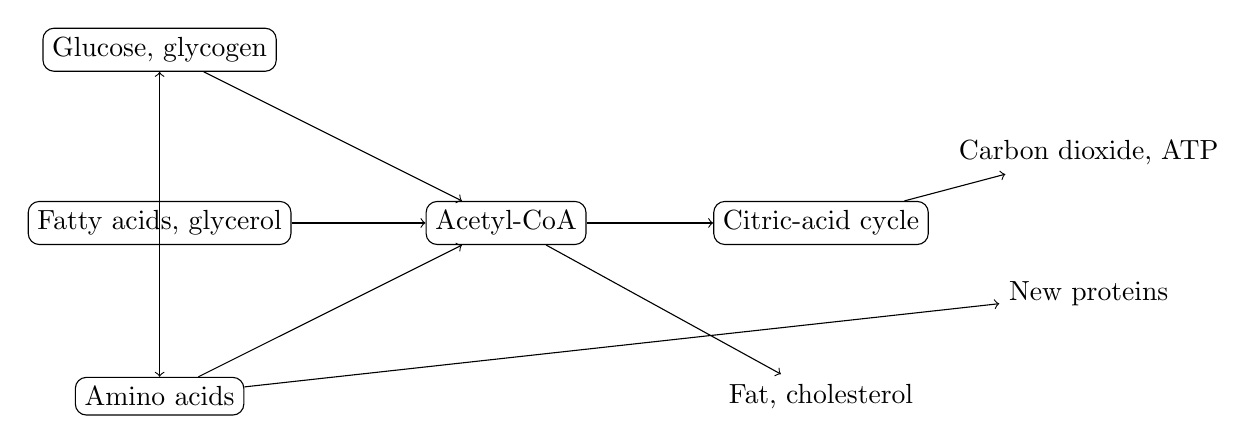
\begin{tikzpicture}
\node[draw, rounded corners] (glu) at (0,2.2) {Glucose, glycogen};
\node[draw, rounded corners] (fa) at (0,0) {Fatty acids, glycerol};
\node[draw, rounded corners] (aa) at (0,-2.2) {Amino acids};
\node[draw, rounded corners] (ac) at (4.4,0) {Acetyl-CoA};
\node[draw, rounded corners] (tca) at (8.4,0) {Citric-acid cycle};
\node (co2) at (11.8,0.9) {Carbon dioxide, ATP};
\node (fat) at (8.4,-2.2) {Fat, cholesterol};
\node (pro) at (11.8,-0.9) {New proteins};
\draw[->] (glu) -- (ac);
\draw[->] (fa) -- (ac);
\draw[->] (aa) -- (ac);
\draw[->] (ac) -- (tca);
\draw[->] (tca) -- (co2);
\draw[->] (ac) -- (fat);
\draw[->] (aa) -- (pro);
\draw[<->] (glu) -- (aa);
\end{tikzpicture}
\end{center}

This is a human representation. Each box represents not one molecule but a continuously entering and leaving population. Arrows mean \textbf{can be converted}, not is being converted now. Box sizes and positions have no relation to a real cell.

\section{Rules: Order Without a Commander}

A city with streets but no traffic lights would soon seize up. Every cell is a metabolic city, with tens of trillions throughout your body and no overall commander. What keeps them orderly?

The first mechanism is \textbf{feedback inhibition}. In a typical synthetic route, raw material A passes through B and C to become product D. When D is plentiful, it returns and binds the enzyme for the route's \textbf{first step}, stopping it. Think of a bakery: when bread fills the shelves, the owner tells the flour mill to stop deliveries instead of letting loaves spoil. Controlling the first rather than last step saves the most: intermediates B and C never accumulate pointlessly.

The second mechanism lies in how D binds. It attaches not at the active site but in another surface pocket. Binding changes the enzyme's overall shape, distorting its active site so the substrate can no longer enter. Binding at a distance to change shape and regulate activity is \textbf{allosteric regulation}, foreshadowed by Chapter 48's flexible protein structures. A molecule need not block the door; a phone call changes the machine's settings.

Third, energy status is itself a signal. Abundant ATP directly allosterically inhibits a key glycolytic enzyme: enough money, stop dismantling glucose. Accumulating ADP and AMP activate the same enzyme: funds are low, speed up. One molecule serves as both currency and dashboard reading. This regulation needs neither hormones nor a brain; it happens inside every cell every second. Chapter 52 said energy status regulates pathways; now you can see the molecular mechanism.

In symbols, for $A \rightarrow B \rightarrow C \rightarrow D$, D inhibits the enzyme catalyzing $A \rightarrow B$. Arrows point right while the signal travels left. Inputs and outputs stabilize production without anyone giving orders.

\section{Evidence: Discovering Constant Bodily Renewal}

\begin{zhengju}
Before the 1930s, the prevailing picture was a house with a stove: the body was already built, while food was burned as fuel. Tissue proteins were considered largely stable, needing only occasional repairs after wear.

The tool that overturned this picture appeared in Chapter 54: isotope tracing, based on Chapter 7's isotope concept. In the early 1930s, scientists isolated deuterium, heavy hydrogen with one extra neutron. Its chemistry is nearly unchanged, but instruments can recognize it. Rudolf Schoenheimer and David Rittenberg at Columbia University immediately saw its value: attach invisible labels to food molecules and follow their destinations in animals.

Their first experiments fed deuterium-containing fatty acids to mice. Days later, the label had not all been burned; much appeared in stored fat, even without weight change. Fat stores were not stationary warehouse inventory but continually deposited, withdrawn, and renewed. A second series went further: after animals ate an amino acid labeled with nitrogen-15, proteins throughout the liver, muscles, and skin carried the label within days. It even appeared in \textbf{other} amino acids, showing interconversion.

Could this be an artifact, such as labels merely sticking to tissue surfaces? Researchers ground the tissue and chemically isolated the proteins before measuring: the labels were inside molecules and could not be washed away. Was turnover limited to active organs like the liver? Muscle and skin proteins also became labeled, only more slowly.

The conclusion appeared in the influential 1942 book ``The Dynamic State of Body Constituents'': \textbf{the body's building materials are continually dismantled and rebuilt}. Stable weight means breakdown and construction balance, not that nothing happens. More precise later measurements refined the picture: turnover differs enormously among tissues. Half the liver's proteins are replaced within days, muscle proteins over weeks, and eye-lens proteins hardly at all during a lifetime. Dynamics are widespread, but rates vary. Today's carbon-13 breath test for Helicobacter pylori uses the same labeling idea.
\end{zhengju}

\section{Rules: Body-Wide Traffic Lights}

Individual cells self-regulate, but liver, muscle, fat, and brain perform different jobs. What tells them whether to store or withdraw fuel? Hormones coordinate the body as chemical messages delivered through blood. The two leading metabolic messengers are \textbf{insulin} and \textbf{glucagon}, both secreted by the pancreas and acting in opposite directions. Chapter 58 explains how their messages enter cells; here we consider what they direct.

\textbf{Just after a meal:} blood glucose rises and insulin responds. It tells muscle and fat cells to open glucose routes and take sugar from the blood, tells liver and muscle to store glucose as glycogen, and tells fat cells to turn surplus materials into fat. Blood glucose falls. In short: the harvest is in; fill the stores.

\textbf{Hours after a meal and overnight:} blood glucose falls and glucagon responds. It tells the liver to break glycogen back into glucose and release it into blood, maintaining supplies to the brain and red blood cells, which recognize almost only glucose. Open the granary, but only the liver's: muscle glycogen is private stock, not for sale.

\textbf{After more than a day without food:} liver glycogen, only about 100 grams and less than a day's supply, runs low, so the body turns to fat. Adipose tissue releases fatty acids for tissues to burn; the liver converts some into ketone bodies as alternative brain fuel. Some muscle protein also breaks down, supplying amino acids for gluconeogenesis. This is why prolonged fasting reduces both muscle and fat.

\textbf{During exercise:} muscles first burn their own glycogen. Within minutes, blood-delivered glucose and fatty acids join in; the longer exercise lasts, the greater the fat contribution. Notice that the proportion changes. Fat contributes from the first minute: there is no switch that starts fat burning only after half an hour. Your muscles resemble a hybrid vehicle, always blending electricity and fuel but adjusting the mix to conditions.

Broken traffic lights cause disease. In type 1 diabetes, the pancreas cannot produce insulin, so the harvest message goes unheard and glucose accumulates in blood instead of entering cells. Blood glucose becomes dangerously high while cells starve, requiring lifelong insulin injections. Another example shows the network's importance: in phenylketonuria, or PKU, an enzyme processing the amino acid phenylalanine is defective. One blocked junction causes upstream phenylalanine accumulation that damages the developing brain. The response is not a drug to repair the enzyme but dietary management: reduce phenylalanine-containing foods so traffic stays below the junction's capacity. Routine newborn heel-prick screening commonly includes PKU; a network map becomes a lifesaving dietary plan. Again, nutrition and medicine depend on dose, evidence, and individual differences. Any claim that a food is good or bad must ask: for whom, and how much?

\textbf{Translator safety note:} The source's PKU treatment account is incomplete: care may include medication as well as an individually prescribed diet. Do not restrict essential amino acids or change medicines on your own. See \href{https://www.nichd.nih.gov/health/topics/pku/conditioninfo/treatments}{NICHD PKU treatment guidance}. People with diabetes must not omit prescribed insulin; diabetic ketoacidosis is a medical emergency requiring immediate care, as explained by \href{https://www.niddk.nih.gov/health-information/diabetes/overview/managing-diabetes}{NIDDK}.

\section{Limits: Where This Map Can Mislead}

The network model is powerful, but overextending it misleads. Remember four limits.

First, arrows mean a conversion is possible, not that it is happening now. The same map carries very different flows in a fed versus fasting body. The drawing is static; the network is alive.

Second, a flat map places everything together, but real cells house pathways in different rooms: glycolysis in the cytoplasm, the citric-acid cycle in mitochondria. The same molecule has different fates in different rooms. Spatial arrangement is a crucial network layer, explored in Chapter 57.

Third, different people have different versions of junction enzymes. Lactose intolerance in Chapter 46 and PKU both reflect innate differences in a junction's capacity. No diet is equally right for everyone: the same network runs with individual parameters.

Fourth, network knowledge cannot yet predict precisely what a particular food will do to you. Blood glucose and cholesterol are only a few windows into the whole network; doctors consider trends and the overall picture, not one number. Any promise to calculate exactly what you should eat exceeds today's evidence.

\begin{wuqu}
``Walnuts nourish the brain, pork skin beautifies skin, and kidneys strengthen kidneys: eating a part strengthens that part.''

This is what happens when metabolism is mistaken for a direct assembly line, as though a dedicated route connected mouth to target organ. In reality, pork-skin collagen is digested into amino acids and enters the body's common amino-acid pool. Those amino acids may become hair, enzymes, or new skin at a wound; alternatively, they may lose their amino groups and be burned into carbon dioxide, or become glucose and fat. No amino acid remembers coming from pork skin, and no mechanism sends it specifically to your face. Likewise, most walnut fat is burned or reassembled for storage, not queued for delivery to the brain.

A counterexample is obvious: strict vegetarians never eat muscle yet still build it. Beans provide amino acids, and the body supplies the blueprint. The defensible kernel of such claims is the ingredient list: some essential amino acids and fatty acids cannot be made by the body and must come from food, as Chapters 46 and 47 explained. Food supplies bricks; the body decides what to build. The construction plan was never in the food.
\end{wuqu}

\section{Another Look at the Rice}

Now check your answer. Three days later, some carbon atoms from the rice have become carbon dioxide exhaled from your lungs. Others remain stored as liver or muscle glycogen, or newly made fat in adipose cells. A small portion has taken a winding route into a protein's carbon skeleton. The pork's proteins became amino acids in the common pool, perhaps repairing muscle or perhaps being burned. They had no express route to your muscles.

Crucially, these proportions are not fixed. The same rice has very different destinations if you sleep after eating or play ball. Its fate depends on the network's current state: inventories, hormonal messages, and your activity. No molecule has a predestined destination, only probabilities and regulation. Unless you guessed that everything went to one place, your original proportions were at least half right.

\section{Going Deeper: Where Does the Network Live?}

Our causal chain is now long: atoms, molecules, reactions, organic molecules, biological macromolecules, and finally this part's theme---organization into a metabolic network that powers, repairs, and regulates itself. Part VI ends here.

But one question may have been building: we keep saying inside cells and mitochondria, but what sort of container holds this network? Why do dozens of reactions and thousands of molecular species crowded into a space narrower than a hair not become chaos? A cell is not a beaker. With internal structures, transport systems, and communication, it is more city than bag. Next part, we enter that city. Chapter 56 asks the biggest question first: how did such a chemical city initially assemble spontaneously from molecules? Chapter 57 tours its districts and logistics. This chapter's flat network will fold into a three-dimensional, breathing city.

\begin{tiaozhan}
Steady state is not equilibrium, a distinction easily confused in metabolism. Chapter 30's chemical equilibrium has equal forward and reverse rates and no \textbf{net} flow. Steady blood glucose instead has equal inflow and outflow with continuous turnover. Picture a bathtub with both tap and drain open: the level stays constant while the water changes. Put numbers in: about 5 liters of blood at about 1 gram of glucose per liter gives 5 grams in total, the water level. During fasting, the liver releases several to more than ten grams per hour, while tissues consume the same amount. At 6 grams per hour, a glucose molecule stays in the pool an average of $5 \div 6 \times 60 = 50$ minutes. The level barely changes, but the contents have been replaced repeatedly: that is dynamic state in quantitative terms. If inflow suddenly exceeds outflow after a large meal, the rising level triggers insulin to increase outflow. Feedback gives the bathtub automatic level control. Any system described by inflow, outflow, and inventory can be approached this way: body temperature, blood calcium, even a city's goods. Skipping this box does not affect the main argument.
\end{tiaozhan}

\section*{Practice}

\begin{sikaoti}
\item Draw a material-flow map for fat and protein in braised pork, from eating through breakdown to the downtown roundabout. From there, draw at least three destinations and label them burning, storage, or building.
\item Use feedback inhibition to explain why eating large amounts of an amino acid does not necessarily make the body produce large amounts of a corresponding protein. Where do excess amino acids ultimately go?
\item Draw blood glucose as a bathtub's water level. Label the inlets and outlets, and explain how insulin adjusts them after a large meal to prevent an excessive rise.
\item A person drinks only water and eats nothing for three days. Describe the fuel-source changes in chronological order and explain why both fat and muscle decrease.

\textbf{Translator safety note:} Treat the three-day fasting scenario as a paper exercise, not an experiment or diet recommendation. Skipping meals or fasting can cause dangerous low glucose, especially with diabetes medicines; consult your care team rather than changing food or medication yourself. See \href{https://www.niddk.nih.gov/health-information/diabetes/overview/preventing-problems/low-blood-glucose-hypoglycemia}{NIDDK hypoglycemia guidance}.

\item Each ATP molecule cycles about 1700 times daily in this chapter's estimate. Calculate its average cycle time in seconds, using about 86000 seconds per day, and explain one fundamental difference between energy currency and paper money.
\item A relative says, ``My skin has been bad lately; I should eat more pig's trotters to improve it.'' Write three sentences using this chapter's model, identifying the mistake while acknowledging any small valid point you can find.
\end{sikaoti}
